\section{Analysis of Coulomb-nuclear interference region}
\label{sec:cni}

\> general note: approach = not just a blind fit, but probe and test

\> key elements of phenomenology/theory of Coulomb-nuclear interference
\>> Coulomb amplitude: ``well'' known
\>> interference formula: SWY (traditionally used) or KL (theoretically more appropriate)
\>> modulus of nuclear amplitude -- strongly constrained by data $\Rightarrow$ exponential parametrisation $\d\sigma / \d t \propto \exp( -B(t) )$; reasonable degrees of the $B(t)$ polynomial are $N_b = 1, 2, 3$ (describes well the data and many phenomenological models); $N_b = 1$ gently disfavoured by the data ($B(t)$ plots, worse fits); fit amplitude anchored to $90\un{m}$ data at $|t| > 0.2\un{GeV^2}$
\>> phase of nuclear amplitude -- weak guidance from data $\Rightarrow$ need assumption: constant, central, peripheral (the last two as from \cite{kl94})

\> two goals
\>> distinction between different models/assumptions: interference formula, phase of nuclear amplitude, degree of the $B(t)$ polynomial. See section \ref{sec:cni dist mod}.

\>> determination of parameters of interest (e.g.~$\rho$, total cross-section with Coulomb taken into account), for certain reasonable models/assumptions. In section \ref{sec:cni par det}.


%-------------------------
\subsection{Parameter determination}
\label{sec:cni par det}

\> general comment: need to work with certain theoretical framework (assumption), the following chosen
\>> with SWY: only constant phase and $N_b = 1$
\>> with KL: nuclear phase constant/central/peripheral, $N_b = 1, 2, 3$ (exclude 1 ??)

\> central/peripheral phases: parametrisations as in \cite{kl94}, but refitted at $8\un{TeV}$ -- some details of the fitting ??
\>> uncertainties of the phase parameters -- {\bf waiting for the input from Vojt\v ech}.


\> generalised $\chi^2$ fits (covariance matrix contained all relevant contributions: statistical, normalisation and misalignment), fits driven by Minuit

\> extensive MC tests (input: phenomenological models as well as data fits)
\>> check for bias: only small
\>> understanding/evaluation of the method response to statistical and systematic uncertainties

\> results ($\rho$, $\sigma_{\rm tot}$, $B^{\rm N}(0)$, ...)
\>> for the model choices above -- keeping phase parameters fixed at their central values from Vojt\v ech
\>> for peripheral-phase parameters being varied within their uncertainties $\Rightarrow$ uncertainty band

\> question: do we want to present a single-value result for $\rho$ (combined from fits under different models) ??

\> discuss the new value of $\sigma_{\rm tot}$ in comparison to our previous measurement \cite{prl111}; values compatible; remind in what is the new measurement better ??

\> reference to Fig.~\ref{fig:rho_s}

\begin{figure*}
\begin{center}
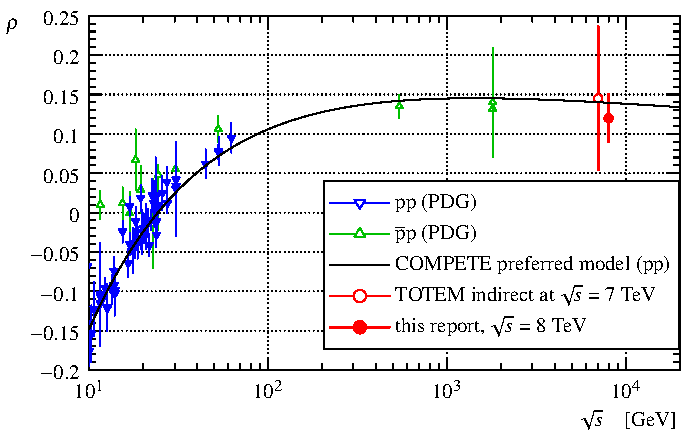
\includegraphics[width=16cm]{fig/rho_s.pdf}
\vskip-3mm
\caption{$\rho$ as a function of $s$.}
\label{fig:rho_s}
\end{center}
\end{figure*}

\> figure for $\sigma_{\rm tot}$ result ?? 

%-------------------------
\subsection{Distinction between different models}
\label{sec:cni dist mod}

\> wish to discriminate between
\>> SWY and KL interference formulae: very little difference predicted, not possible with the current data (prove/illustrate)
\>> constant/central phase: very little difference predicted, not possible with the current data (prove/illustrate)
\>> constant/peripheral phase: gentle (percent) effect at higher-$|t|$ region
\>> degree of the $B(t)$ polynomial

\> match metrics: Kolmogorov-like (explain!). Integration from right optimises sensitivity in higher-$|t|$ region where the effect of different phases is more significant (as opposed to the low-$|t|$ region mostly sensitive to $\rho$)
\>> why not using $\chi^2$: all points mixed $\Rightarrow$ not enough sensitivity

\> minimisation engines: custom developed simplex minimisation with simulated annealing (according to the Numerical Recipes)
\>> scans used to validate the algorithm

TODO: the rest

